%&latex
%
\documentclass[../template.tex]{subfiles}
\usepackage{graphicx}

\begin{document}

\subsection{Remark on the Legendre Transform}
We saw that the \textit{Free energy} $A(T,V,N)$ is the Legendre transform of the \textbf{energy} with respect to the \textbf{entropy}:
\begin{align}
    \dd{\mathcal{E}} &= - P\dd{V} + T \dd{S} + \mu \dd{N} \label{eqn:60}\\
    \left(\pdv{\mathcal{E}}{S}\right)_{VN} &= \mathcal{E}- TS \label{eqn:61}
    \shortintertext{Then we solve for $S(T,V,N)$ and write}:
    A(T,V,N) &= \mathcal{E} - TS \label{eqn:62}\\
    \dd{A} = - P\dd{V} -S \dd{T} + \mu \dd{N} \label{eqn:63}\\
    \left(\pdv{A}{N}\right)_{VT} &= \mu \label{eqn:64}
    \shortintertext{And we solve for $N(T,\mu,V)$. The Legendre transform of $A$ wrt $N$ (or equivalently the Legendre transform of $E$ wrt both $S$ and $N$) is:}
    \Phi(T,\mu,V) &= A - N \mu \label{eqn:65}\\
    \dd{\Phi} &= - P\dd{V} - S\dd{t} - N \dd{\mu} \label{eqn:66}
    \shortintertext{Note that $\Phi$ is extensive since $A$ and $N$ are, and so $\Phi(T, \mu, V) = V\varphi(T, \mu)$. Then:}
    -P &= \left(\pdv{\Phi}{V}\right)_{T,\mu} = \varphi(T,\mu)\\
    \Phi(T,\mu,V) &= -P(T,\mu) V \label{eqn:67}
\end{align}
where $P(T,\mu)$ is the \textit{grand-canonical} pressure.

\begin{exo}[4]
    Determine $\Phi$ for the Ideal Gas and show that:
    \begin{align*}
        P(T,\mu) V = \langle N \rangle k_B T
    \end{align*}
    which is the equation of state in the GC ensemble.
\end{exo}

\subsection{Fluctuation of the number of particles}
This is related to the correction of the saddle-point approximation.
\begin{align}\label{eqn:68}
    e^{\beta PV} &\underset{\substack{(\ref{eqn:44})\\(\ref{eqn:49})}}{=} \sum_N e^{\beta \mu N - \beta A(T,V,N)} =\\ \nonumber
    &\underset{V \gg 1}{=}  e^{\beta \bar{N} \mu - \beta A (T, V, \bar{N})} \int \dd{N} \exp\left(-\frac{(N-\bar{N})^2}{2 \sigma_N^2} \right) + \dots
\end{align}
where:
\begin{align}\label{eqn:69}
    \sigma_N^2 = \langle (N-\bar{N})^2 \rangle = \left(\beta \pdv[2]{A}{N}\right)^{-1}_{N = \bar{N}}
\end{align}

Since from exercise 3 above we have:
\begin{align}\label{eqn:70}
    A(T,V,N) = N a(T,v) + O(\ln N) \qquad v=\frac{V}{N} 
\end{align}
(In the following the subindex \textit{c} refers to \q{Canonical Ensemble}).

\begin{align}\label{eqn:71}
    \left(\pdv[2]{A}{N}\right)_{\bar{N}} &= \pdv{N} \underbrace{\left[a - v \pdv{a}{v}\right]}_{\pdv{A}{N} \equiv \mu_c (T,v)}\Big|_{\bar{N}} = - \frac{v^2}{V} \pdv{v} \mu_c(T,V)\Big|_{\bar{v}} =\frac{v^3}{V} \pdv[2]{a}{v}\Big|_{\bar{v}} =\\ \nonumber
    &= -\frac{v^3}{V} \pdv{P_C}{v} \Big|_{v = \bar{v}} \qquad \bar{v} \equiv \frac{\bar{N}}{V} 
\end{align}
where we have used:
\begin{align}\label{eqn:72}
    P_c \underset{(\ref{eqn:63})}{=} -\pdv{A}{V} = -\pdv{a}{v}
\end{align}
From equations (\ref{eqn:69}) and (\ref{eqn:71}) we have:
\begin{align} \label{eqn:73}
    \sigma_N^2 = \frac{k_B T V}{\bar{v}^2} k_T = \bar{N} \frac{k_B T}{\bar{v}} k_T \Rightarrow \frac{\sigma_N}{\sqrt{\bar{N}}}    \propto \frac{1}{\sqrt{\bar{N}}} 
\end{align}
where:
\begin{align}\label{eqn:74}
    k_T \equiv \bar{v} \left(-{\pdv{P_c}{v}}(T,v)\right)_{\bar{v}}
\end{align}
is the \textbf{isothermal compressibility}.

\begin{exo}[5]
    Show that in the special example of the Ideal Gas we have:
    \begin{align}\label{eqn:75}
        k_T(T,v) = \frac{k_B T}{v} 
    \end{align}
\end{exo}

In chapter $2$ we found the energy fluctuation in the canonical ensemble to be:
\begin{align}
    \label{eqn:76}
    \sigma_{\mathcal{E}}^2 = \langle (H- \langle H \rangle)^2 \rangle = k_B T^2 C_v(T,V,N) \Rightarrow \frac{\sigma_F}{\langle H \rangle}  \propto \frac{1}{\sqrt{N}} 
\end{align}
where $C_V$ is the heat capacity ($\propto N$).

Equations (\ref{eqn:74}) and (\ref{eqn:76}) are two instances of the famous fluctuation dissipation theorem (another instance is the Einstein relation we found in chapter $4$).

In both cases above we see that the fluctuations $\sigma_N/\langle N \rangle$ and $\sigma \mathcal{E}/\langle H \rangle$, ($\langle H \rangle \propto N$) tend to $0$ in the thermodynamic limit unless the isothermal compressibility and the heat capacity diverges. Typically this is what happens at a phase transition as we will see in the next chapter.

\subsection{Absence of macroscopic motion in equilibrium}
The MaxEnt principle allows us to prove that in equilibrium there cannot exist macroscopic motion of matter. Indeed, divide the $3D$ system in macroscopically small regions such that \textit{at stationarity} the part of the system occupying the $j$-th cell has a momentum $\bm{p}_j$, a mass $M_j$, a total energy $\mathcal{E}_j$ and thus an internal energy:
\begin{align*}
    E_j - \frac{P_j^2}{2 M_j} = E_j^{\mathrm{Internal}} 
\end{align*} 
and an entropy:
\begin{align*}
    S_h(E_j - P_j^2/(2M_j))
\end{align*}

\begin{figure}[H]
    \centering
    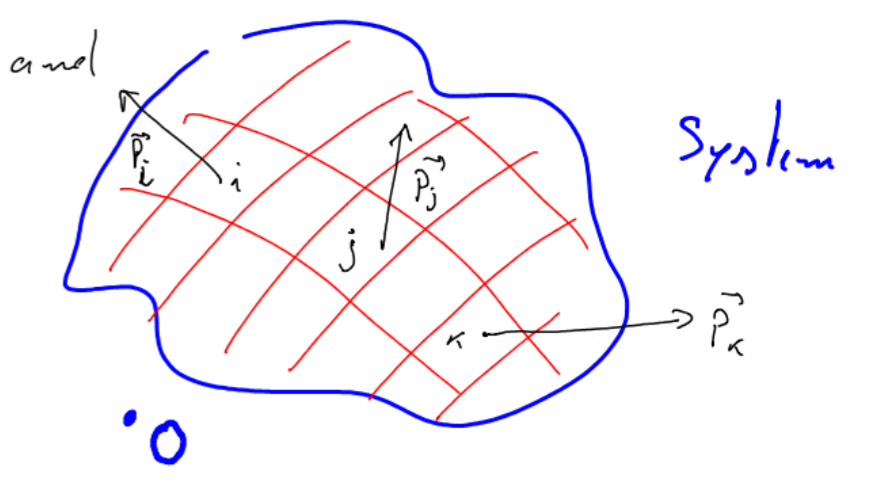
\includegraphics{image005.png}
    \caption{Each macroscopic region of the system at equilibrium shares the same momentum and angular momentum.\label{fig:macmov}}
\end{figure}

We assume that the volume of the cell is fixed and also the number of particles that it contains (thus we will not display their dependence in $S_j$). If interparticle forces are short range, the total entropy is:
\begin{align}\label{eqn:77}
    S = \sum_j S_j\left(\mathcal{E}_j - \frac{P_j^2}{2 M_j} \right)
\end{align}
The system is isolated and so:
\begin{align}\label{eqn:78}
    \sum_j \mathcal{E}_j = \mathcal{E}, \quad \sum_j \bm{p_j} = \bm{P}, \quad \sum_j \bm{r_j} \times \bm{P_j} = \bm{L}
\end{align}
are conserved but otherwise undetermined. Assuming the MaxEnt principle we have to maximize $S$ wrt $\bm{p_j}$ under the $7$ constraints (\ref{eqn:78}), and so we have to determine the stationary conditions for the following system:
\begin{align*}
    \mathcal{F} = \sum_j S_i \left(\mathcal{E}_j - \frac{P_j^2}{2 M_j} \right) + \bm{a} \sum_j \bm{p_j} + \bm{b} \sum_j \bm{r_j} \times \bm{p_j} - c \sum_j \mathcal{E}_j
\end{align*}
\begin{align}\label{eqn:79}
    \pdv{\mathcal{F}}{\mathcal{E}_j} = 0 \Leftrightarrow \pdv{S_j}{E_j} \left(\mathcal{E}_j - \frac{P_j^2}{2M_j} \right) = c \quad \forall j
\end{align}
%which this identify with $1/T$, as usual

\begin{align}\label{eqn:80}
    \grad_{\bm{p_j}} \mathcal{F} = 0 \Leftrightarrow \underbrace{\pdv{E_j} S_j \left(\mathcal{E}_j - \frac{P_j^2}{2 M_j} \right)}_{1/T} \qquad \frac{\bm{p_j}}{M_j} = \bm{a} + \bm{b} \times \bm{r_j}
\end{align}

\begin{align}\label{eqn:81}
    \bm{v_j} = \frac{\bm{p_j}}{M_j} = (\bm{a} + \bm{b} \times \bm{r_j}) T
\end{align}
which tells us that all parts have a common uniform translation velocity $\bm{a}T$ and a uniform rotatory motion with angular velocity $\bm{\Omega} = \bm{b}T$. Thus the system behaves like a rigid body as far as the macroscopic motion is concerned.

\medskip

$\operatorname{He}^4$ is exceptional since it cannot rigidly rotate.

\begin{figure}[H]
    \centering
    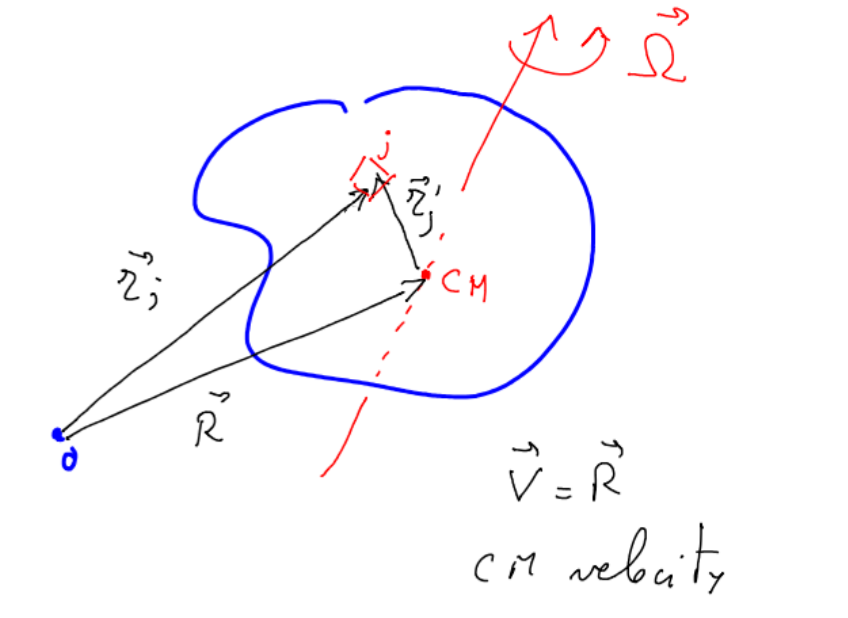
\includegraphics{image006.png}
    \caption{\label{fig:rotations}}
\end{figure}

\begin{align*}
    \bm{r_j} &= \bm{R} + \bm{r_j'}\\
    \bm{v_j} &= \dot{\bm{r}}_{\bm{j}} = \dot{\bm{R}} + \dot{\bm{r}}'_{\bm{j}} = \bm{V} + \bm{\Omega} \times \bm{r}'_j = \underbrace{\bm{V} - \bm{\Omega} \times \bm{R}}_{\bm{a}T} + \underbrace{\bm{\Omega} \times \bm{r_j}}_{\bm{b}T}
\end{align*}

\section{Non Equilibrium Entropy}
May we define the entropy in non equilibrium like we did in (\ref{eqn:7b}).
\begin{align}\label{eqn:82}
    S_I[\rho(t)] = -k_B \int \dd{\Gamma} \rho(\mathbb{Q}, \mathbb{P}, t) \ln \rho(\mathbb{Q}, \mathbb{P},t)
\end{align}
where the non-equilibrium probability distribution is time independent and, of course, satisfies the Liouville Theorem (\ref{eqn:6}, ch. 5):

\begin{align}\label{eqn:83}
    \pdv{t} \rho(\mathbb{Q}, \mathbb{P}, t) &= - \sum_\alpha \left[{\pdv{\rho}{q_\alpha}}(\mathbb{Q}, \mathbb{P},t) {\pdv{H}{p_\alpha}}(\mathbb{Q}, \mathbb{P}) - {\pdv{\rho}{p_\alpha}}(\mathbb{Q}, \mathbb{P}, t) {\pdv{H}{q_\alpha}}(\mathbb{Q}, \mathbb{P}) \right] =\\
    &\equiv -\{\rho, H\} \nonumber
\end{align}
with a given initial condition $\rho(\mathbb{Q}, \mathbb{P}, t=0)$.

\medskip

Let us consider our paradigm of irreversible transformation:

\begin{figure}[H]
    \centering
    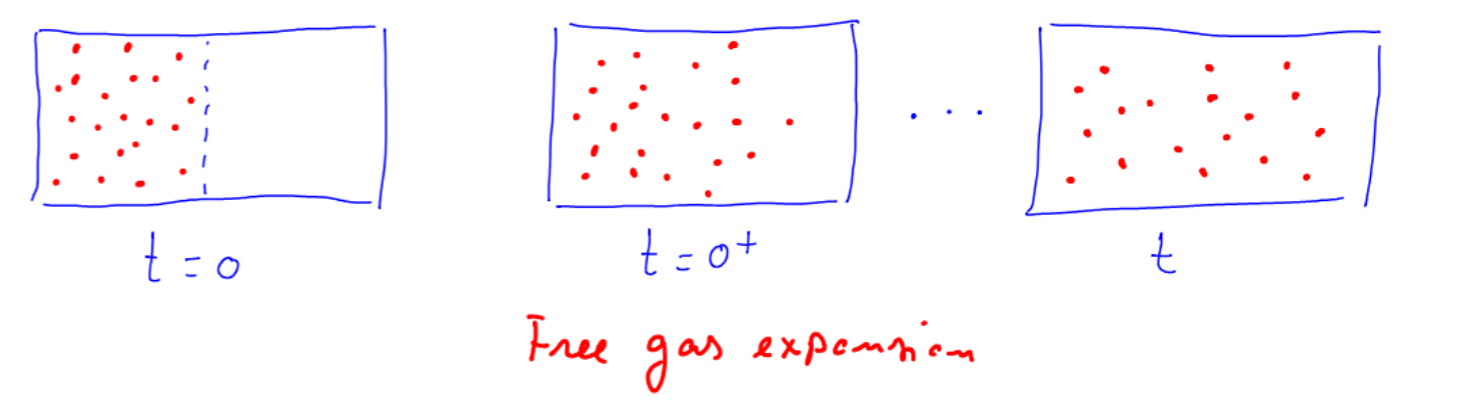
\includegraphics{image004.png}
    \caption{Irreversible transformation: free gas expansion.\label{fig:irrev}}
\end{figure}
and let us calculate $\dd{S_I}/\dd{t}$ using (\ref{eqn:82}) and (\ref{eqn:83}) (compare with exercise 5.7 of Sethna).

For a generic functional $F$ ($S_I$ is a particular instance):
\begin{align}\label{eqn:84}
    F[\rho] = \int f(\rho(\mathbb{Q}, \mathbb{P}, t)) \underbrace{\dd[3N]{\mathbb{Q}} \dd[3N]{\mathbb{P}}}_{\dd{\Gamma}} 
\end{align}
we have:
\begin{align}\label{eqn:85}
    \dv{t} F[\rho] &= \int \pdv{t} f(\rho(\mathbb{Q}, \mathbb{P},t)) \dd{\Gamma} = \int \dd{\Gamma} f'(\rho) \pdv{r}{t} =\\ \nonumber
    &\underset{(\ref{eqn:83})}{=} -\int \dd{\Gamma} f'(\rho) \grad \rho \cdot \mathbb{V} = -\int \dd{\Gamma} \grad f(\rho) \cdot \mathbb{V}\\
    \grad \rho &= \left(\pdv{\rho}{q_\alpha}, \pdv{\rho}{p_\alpha}\right)^T \in \mathbb{R}^{6N} \label{eqn:86}\\
    \bm{V} &= \left(\pdv{H}{p_\alpha}, -\pdv{H}{q_\alpha}\right)^T \in \mathbb{R}^{6N} \label{eqn:87}
\end{align}
Notice that:
\begin{align}\label{eqn:88}
    \grad \cdot \bm{\mathbb{V}} = \sum_\alpha \left(\pdv{q_\alpha} \pdv{H}{p_\alpha} - \pdv{p_\alpha} \pdv{H}{q_\alpha}\right) = 0 \\
    \Rightarrow \grad f \cdot \bm{\mathbb{V}} = \grad \cdot (f \bm{\mathbb{V}}) - f \grad \cdot \bm{\mathbb{V}} = \grad (f \bm{\mathbb{V}}) \span \label{eqn:89}
\end{align}
Thus (\ref{eqn:85}) becomes:
\begin{align}\label{eqn:90}
    \dv{t} F[\rho] = -\int \dd{\Gamma} \grad (f \bm{\mathbb{V}}) = - \oint_{\parbox{3em}{$\,\,$\scriptsize Surface in $\Gamma$ at $\infty$}} \dd{\bm{\Sigma}} \cdot \bm{\mathbb{V}} f = 0
\end{align}
In our case $f(\rho) = -k_B \rho \ln \rho$. Since $\int \rho \dd{\Gamma} = 1$, then $\rho \to 0$ when $\mathbb{Q}, \mathbb{P} \to \infty$ and so $f(\rho) \to 0$ on the surface at $\infty$ in the last integral. In summary:
\begin{align}\label{eqn:91}
    \dv{t} S_I[\rho(t)] = 0
\end{align}
that is the information entropy does not change in the irreversible process of the free expansion (and any other process!). 

\medskip

This is because $\rho$ encodes \textit{full information} about the system, and during the deterministic evolution we do not lose any of it, meaning that our \textit{ignorance} does not rise.

\medskip

If we \textit{discard} some of the information, we will see the entropy rise. For example, consider the marginal probability distribution $\rho_D(\mathbb{Q}, t)$, and suppose it evolves as a diffusion process:
\begin{align} \label{eqn:93}
    \dot{\rho}_D(\mathbb{Q},t) = D \nabla^2 \rho_D(\mathbb{Q},t)
\end{align} 
We now compute:
\begin{align*}
    dv{t} S_I[\rho_D(t)] &= -k_B \dv{t} \int \rho_d \ln \rho_d \dd[3N]{\mathbb{Q}} = \\
    &= -k_B \int \left[\pdv{\rho_D}{t} \ln \rho_d + \rho_d \pdv{\rho_d}{t} \frac{1}{\rho_d} \right] \dd[3N]{\mathbb{Q}}
\end{align*}
Note that the last term:
\begin{align*}
    -k_B \int \dd[3N]{\mathbb{Q}} \pdv{t} \rho_D(\mathbb{Q},t) = -k_B \pdv{t} \underbrace{\int \dd[3N]{\mathbb{Q}} \rho_D(\mathbb{Q},t)}_{=1} = 0 
\end{align*}
Thus:
\begin{align}\label{eqn:94}
    \dv{t} S_I[\rho_D(t)] &= -k_B \int \dd[3N]{\mathbb{Q}} \pdv{t} \rho_D \ln \rho_D = \\
    &= -k_B D \int \dd[3N]{\mathbb{Q}} (\nabla^2 \rho_D) \ln \rho_D = k_B D \int \dd[3N]{\mathbb{Q}} \frac{(\grad \rho_D)^2}{\rho_D} \geq 0 
\end{align}
where we have integrated by parts and assumed that $(\grad \rho_D) \ln \rho_D \to 0$ when $\mathbb{Q} \to \infty$. This is due to the fact that $-D \grad \rho_D$ is the probability flux and this has to be $0$ at infinity if the probability has to be conserved. Then:
\begin{align}\label{eqn:95}
    0 = \pdv{t} \int \rho_D \dd[3N]{\mathbb{Q}} = D \int \nabla^2 \rho_D \dd[3N]{\mathbb{Q}} =D \int \dd{\bm{\Sigma}} \cdot \grad \rho_0
\end{align}
As expected, now the entropy \textit{rises} during the irreversible transformation.

\medskip

Clearly, the diffusion assumption is \textit{ad-hoc}. To obtain a definition of entropy for the non-equilibrium case which is truly general we need a different approach altogether. One possible way is to divide the system in macroscopically small parts, so that each of them $\dd[3]{\bm{r}}$, has a well defined energy density $\epsilon(\bm{r},t)$, number of particles density $n(\bm{r},t)$ and velocity $u(\bm{r},t)$ and so it can be considered \q{in equilibrium}. This is, in essence, the hypothesis of \textbf{local thermal equilibrium} (lte).

\medskip

Recall that, for a macroscopic system, we have:
\begin{align}\label{eqn:96}
    S(\mathcal{E}, V, N) = V s\left(\frac{\mathcal{E}}{V}, \frac{N}{V}  \right)
\end{align}
This suggests to define the entropy of the system outside equilibrium but in lte (and with short range interparticle forces) as:
\begin{align}\label{eqn:97}
    S(\epsilon, n, u) = \int \dd[3]{\bm{r}} s\Big(\underbrace{\epsilon(\bm{r},t) - \frac{m}{2} u^2(\bm{r},t)}_{\parbox{7em}{\centering\scriptsize Internal energy of the subsystem in $\dd[3]{\bm{r}}$ centred at $\bm{r}$}} , n(\bm{r},t) \Big)
\end{align}
This $S$ \textit{never decreases} over time!

Notice that (\ref{eqn:97}) does not take into account all the details of the evolution like it did $S_I[\rho]$. Thus the set of configurations $(\mathbb{Q}, \mathbb{P})$ at time $t$ which derives from initial configurations at time $t=0$ where all the particles were on the left side of a box have an essentially zero measure (from the Liouville theorem) and thus when included in (\ref{eqn:97}) have the same $\epsilon(\bm{r},t)$, $u(\bm{r},t)$, $n(\bm{r},t)$ as the almost totality of configurations that will \q{never} have the possibility to lead the gas again the left half of the box once the momenta $\mathbb{P} \to -\mathbb{P}$. This means that even changing $t \to -t$ will make $S$ in (\ref{eqn:97}) to decrease in time.

\subsection{Maxwell demon}

\begin{figure}[H]
    \centering
    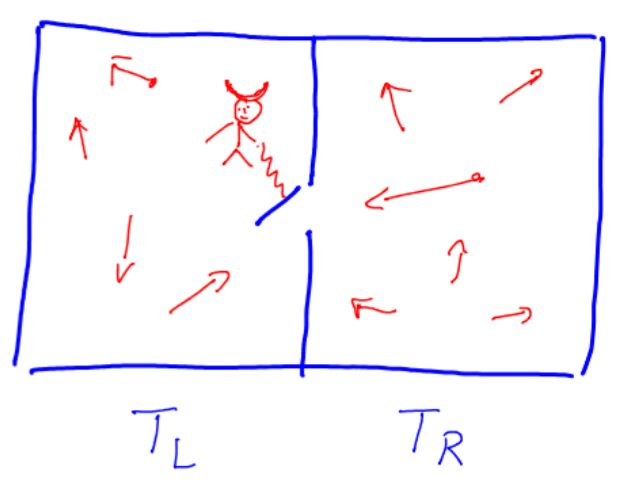
\includegraphics{image007.png}
    \caption{\label{fig:maxwell}}
\end{figure}

The demon is a device that allows fast particles from the right to go to the left. 
\begin{align*}
    0 \leq \Delta S_{\mathrm{tot}} = \underbrace{\Delta S_{\mathrm{env}} + \Delta S_{\mathrm{sys} }}_{\text{might be $\leq 0$}}  + \Delta S_{\mathrm{demon}}
\end{align*}
The second principle of thermodynamics may appear violated when considering only the system and the environment. However, it must apply when we consider also the \textit{demon}. In other words, the act of storing information (or, more precisely, \textit{deleting it}), produces entropy. 
See ex. 5.2.

\end{document}
